
\chapter{CTL下的遗忘理论的定义及其语义属性}\label{chapter03}
{\em 本章首先通过扩展互模拟的概念,给出$\CTL$下遗忘理论的定义。其次,探索遗忘理论的一般通用属性,这些属性包括:模块化(Modularity)性质、交换性(Commutativity)、齐次性(Commutativity)等属性。}

\section{引言}
从一个公式中“遗忘”掉一些原子命题得到的结果应该不违背定义在剩余原子命题集合上的公式,也就是说对于剩余原子命题集合上的公式,原始公式能够逻辑蕴涵它当且仅当遗忘得到的结果能过逻辑蕴涵它。从模型的角度来讲,遗忘得到的结果的模型与原始公式的模型在除去被遗忘的那些原子命题之后是能够想互模拟的。\emph{互模拟}描述的是两个在行为上能够相互替代的转换系统\cite{Baier:PMC:2008}。在本文中,转换系统被描述成为Kripke结构。因此为了描述遗忘理论,这部分给出在给定原子命题集合上的Kripke结构(或$\Ind$-结构)上的互模拟的定义及其性质。

基于互模拟的概念,给出了$\CTL$下遗忘理论的定义。与后面章节将要讲述的约束$\CTL$下的遗忘相对应,这部分探索没有约束的遗忘理论的一般属性。

\section{$V$-互模拟}

这部分给出定义在给定原子命题集合$V$上的互模拟的概念,本文称之为$V$-互模拟。尽管在文章~\cite{Yan:AIJ:2009}中给出了相似的概念,但是如在基础知识部分所述,$S5$的语义是定义在一种特殊的Kripke结构($\MPK$-解释)下的,因而不具有一般性。接下来探讨一种更加一般的$V$-互模拟。

为此,首先给出能够描述一定深度$n\in \mathbb{N}$的计算树之间的$V$-互模拟关系,记为$\Hb_n^V$。令$V\subseteq \Ha$是原子命题的集合,$i\in \{1,2\}$,$\Hm_i=(S_i,R_i,L_i,s_0^i)$(或$\Hm_i=(S_i,R_i,L_i,[\_]_i,s_0^i)$)是初始结构($\Ind$-Kripke结构),${\cal K}_i=(\Hm_i, s_i)$是$\MPK$-结构(或$\Ind$-结构)。$\Hb_n^V$被递归定义如下:
\begin{itemize}
	\item 若$L_1(s_1)-V=L_2(s_2)$,则$({\cal K}_1,{\cal K}_2) \in \Hb_0^V$;
	\item 对任意$n\ge 0$,若满足下面几个条件,则$({\cal K_1},{\cal K_2})\in \Hb_{n+1}^V$成立:
		\begin{itemize}
			\item $({\cal K}_1,{\cal K}_2) \in \Hb_0^V$;
			\item 对任意$(s_1,s_1')\in R_1$,存在$(s_2,s_2')\in R_2$使得$({\cal K}_1',{\cal K}_2') \in \Hb_n^V$;
			\item 对任意$(s_2,s_2')\in R_2$,存在$(s_1,s_1')\in R_1$使得$({\cal K}_1',{\cal K}_2') \in \Hb_n^V$。
		\end{itemize}
\end{itemize}
其中${\cal K}_i'=(\Hm_i,s_i')$。

当所谈及的原子命题的集合$V$很显然的时候,上述$\Hb_n^V$中的$V$可以省略,记为$\Hb_n$。此外,当讨论的$\Hm_i$$(i=1,2)$是显然的时候,可以使用$(s_1,s_2) \in \Hb_n$代替$((\Hm_1,s_1),(\Hm_2,s_2)) \in \Hb_n$。
此时,$V$-互模拟关系就可以定义如下:
\begin{definition}[$V$-互模拟]\label{def:V-bisimulation}
	令$V$是$\Ha$的一个子集,$i\in \{1,2\}$, ${\cal K}_1$和${\cal K}_2$是$\MPK$-结构(或$\Ind$-结构)。
	\begin{itemize}
		\item ${\cal K}_1$和${\cal K}_2$是$V$-互模拟的,当且仅当对所有的$n \ge 0$都有$({\cal K}_1, {\cal K}_2)\in \Hb_n$。若${\cal K}_1$和${\cal K}_2$是$V$-互模拟的,则记为${\cal K}_1 \lrto_V {\cal K}_2$。
		\item 对$\Hm_i$上的路径$\pi_i=(s_{i,1},s_{i,2},\dots)$,若对于任意的$j\in \mathbb{N}_{\ge 1}$都有${\cal K}_{1,j} \lrto {\cal K}_{2,j}$,则$\pi_1 \lrto_V \pi_2$。其中${\cal K}_{i, j}=(\Hm_i, s_{i,j})$。
	\end{itemize}
\end{definition}

上述$V$-互模拟的定义是现有互模拟定义的一般化,这可以从下面几个方面来体现\footnote{在其他领域也有类似的定义,如:定义在数据库相关文献中的概念$k$-互模拟\cite{kaushik2002updates}。$k$-互模拟概念中涉及与本文$\Hb_n$类似的定义,只是其关系是从相反的方向(即:从孩子到父节点的方向)来说明的。此外,值得一提的是,本文的$V$-互模拟的概念是定义在$\MPK$-结构上的。}。
首先,当给定的$V$为空集且谈论指定的初始状态时,本文的$V$-互模拟与定义在Baier等文章里的互模拟等价(定义7.1\cite{Baier:PMC:2008})的概念一致。
其次,在同一文章里的基于状态的互模拟(定义7.7\cite{Baier:PMC:2008})是定义在给定结构的状态上的,因此与本文的$V$-互模拟(定义在结构的集合上)也不同。
最后,本文的$\Hb_n$的定义与Browne的论文中的状态等价$E_n$类似,只是后者是定义在状态上\cite{browne1988characterizing}而本文的定义在$\MPK$-结构(或$\Ind$-结构)上。


下面例子呈现结构之间的$V$-互模拟。
\begin{example}\label{exam:vB}
	令${\cal K}_1$,${\cal K}_2$和${\cal K}_3$为三个$\MPK$-结构,其图表示分别如图中的${\cal K}_1$,${\cal K}_2$和${\cal K}_3$所示。它们之间的互模拟关系也如图中标记所示,即${\cal K}_1 \lrto_{\{sp\}} {\cal K}_2$,${\cal K}_2 \lrto_{\{se\}} {\cal K}_3$和${\cal K}_1 \lrto_{\{sp,se\}} {\cal K}_3$。此外,可以看出${\cal K}_1$,${\cal K}_2$和${\cal K}_3$之间是互不互模拟\cite{Baier:PMC:2008}的,即不$\emptyset$-互模拟。
	\begin{figure*}[!htb]
		\centering
		% Requires \usepackage{graphicx}
		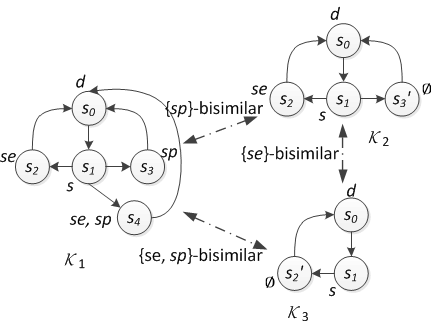
\includegraphics[width=8cm]{chapter03/NVBnewCar.png}\\
		\caption{$\MPK$-结构之间的$V$-互模拟关系}
		\label{Fig:chapter05:v1uv2}
	\end{figure*}
\end{example}

 为了简化书写和看起来简洁,当从上下文中能明确知道所指的初始结构和$\Ind$-Kripke结构(为了方便,将这两种结构通称为结构),则可以使用状态来表示这些结构之间的$V$-互模拟,即使用$s_1 \lrto_V s_2$替代$(\Hm_1, s_1)\lrto (\Hm_2,s_2)$。
 
 $V$-互模拟给出了两个结构之间相互模仿的行为关系,下面的命题给出了这种关系一些关键的性质。
 \begin{proposition}\label{pro:div}
 	令$i$是属于集合$\{1,2\}$的变量,$V_1$和$V_2$是$\Ha$的子集,$s_1'$和$s_2'$是两个状态,$\pi_1'$和$\pi_2'$是两条路径,${\cal K}_j=(\Hm_j,s_j)$$(j=1,2,3)$是$\MPK$-结构(或$\Ind$-结构)。如果$({\cal K}_1 \lrto_{V_1} {\cal K}_2)$且$({\cal K}_2 \lrto_{V_2} {\cal K}_3)$,则:
 	\begin{itemize}
 		\item[] (i) 若$s_1' \lrto_{V_i} s_2'$,则$s_1'\lrto_{V_1 \cup V_2} s_2'$;
 		\item[] (ii) 若$\pi_1' \lrto_{V_i} \pi_2'$,则$\pi_1'\lrto_{V_1 \cup V_2} \pi_2'$;
 		\item[] (iii) 对$\Hm_1$上的任意一条路径$\pi_{s_1}$,存在$\Hm_2$上的一条路径$\pi_{s_2}$使得$\pi_{s_1} \lrto_{V_1} \pi_{s_2}$;反之亦然;
 		\item[] (iv) ${\cal K}_1 \lrto_{V_1 \cup V_2} {\cal K}_3$;
 		\item[] (v) 若$V_1 \subseteq V_2$,则${\cal K}_1 \lrto_{V_2} {\cal K}_2$。
 	\end{itemize}
 \end{proposition}
\begin{proof}
	这里给出结构为$\MPK$-结构的证明,结构为$\Ind$-结构的情形可以类似地证明。
	
	(i) 假设$s_1'$和$s_2'$分别来源于$\Hm_1$和$\Hm_2$,${\cal K}_1=(\Hm_1,s_1)$,${\cal K}_2=(\Hm_2,s_2)$。为了证明$s_1'\lrto_{V_1 \cup V_2} s_2'$,只需证明对于任意的$n\ge 0$,$(s_1',s_2')\in \Hb_n^{V_1 \cup V_2}$。
	
	基始. 当$n=0$时显然是成立的。
	
	归纳步骤. 假设对于任意的$0\leq k \leq n$,若$({\cal K}_1, {\cal K}_2) \in \Hb_k^{V_1}$且$({\cal K}_1, {\cal K}_2) \in \Hb_k^{V_2}$,则$({\cal K}_1, {\cal K}_2) \in \Hb_k^{V_1\cup V_2}$。这里根据定义~\ref{def:V-bisimulation}证明对于若$({\cal K}_1, {\cal K}_2) \in \Hb_{n+1}^{V_1}$且$({\cal K}_1, {\cal K}_2) \in \Hb_{n+1}^{V_2}$,则$({\cal K}_1, {\cal K}_2) \in \Hb_{n+1}^{V_1\cup V_2}$。
	
	(a)$L_1(s_1)-(V_1\cup V_2) = L_2(s_2) - (V_1 \cup V_2)$是显然成立的。
	
	(b)给定$i\in \{1,2\}$,$0< k \leq n+1$,${\cal K}_i^k=(\Hm_i, s_i^k)$。这里将证明对于任意的$(s_1,s_1^1)\in R_1$,存在一个$(s_2,s_2^1)\in R_2$使得$(s_1^1,s_2^1)\in \Hb_n^{V_1\cup V_2}$。
	有归纳假设可知$({\cal K}_1,{\cal K}_2)\in \Hb_n^{V_1\cup V_2}$,因而有$({\cal K}_1^1, {\cal K}_2^1) \in \Hb_{n-1}^{V_1 \cup V_2}$。
	因此,只需证明对于任意的$(s_1^n,s_1^{n+1})\in R_1$,存在$(s_2^n,s_2^{n+1}) \in R_2$使得$(s_1^{n+1},s_2^{n+1})\in \Hb_0^{V_1\cup V_2}$。
	因为$({\cal K}_1,{\cal K}_2)\in \Hb_{n+1}^{V_1}$且$({\cal K}_1,{\cal K}_2)\in \Hb_{n+1}^{V_2}$,所以有$L_1(s_1^{n+1}) - (V_1 \cup V_2) = L_1(s_2^{n+1}) - (V_1 \cup V_2)$。
	
	(c)定义中的第三点可以类似(b)证明。
	
	因此,当令$s_1$和$s_2$分别为$s_1'$和$s_2'$,就可得到$s_1'\lrto_{V_1 \cup V_2} s_2'$。
	
	(ii) 根据定义和(i)很容易证明。
	
	(iii) 为了证明该结论成立,下面给出一个等价的$V$-互模拟的定义。令$V$是$\Ha$的一个子集,${\cal K}_i=(\Hm_i, s_i)$ $(i=1,2)$是$\MPK$($\Ind$)-结构,则${\cal K}_1\lrto_V {\cal K}_2$(也记为$({\cal K}_1,{\cal K}_2) \in \Hb$)当且仅当
	\begin{itemize}
		\item[(a)] $L_1(s_1)-V = L_2(s_2)-V$;
		\item[(b)] 对任意的$(s_1,s_1')\in R_1$,存在一个$(s_2,s_2')\in R_2$使得${\cal K}_1' \lrto_V {\cal K}_2'$;
		\item[(c)] 对任意的$(s_2,s_2')\in R_2$,存在一个$(s_1,s_1')\in R_1$使得${\cal K}_1' \lrto_V {\cal K}_2'$。
	\end{itemize}
	其中${\cal K}_i'=(\Hm_i, s_i')$。

	下面从两个方面证明上述结论成立。
	
	($\Rto$) (a) 显然$L_1(s_1)-V = L_2(s_2)-V$成立。
	
	(b) ${\cal K}_1 \lrto_V {\cal K}_2$当且仅当对于所有的$n\ge 0$都有$({\cal K}_1, {\cal K}_2)\in \Hb_n$。因此,对任意的$(s_1,s_1')\in R_1$,存在一个$(s_2,s_2')\in R_2$使得对于任意的$n >0$都有$({\cal K}_1', {\cal K}_2') \in \Hb_n$且$L_1(s_1')-V=L_2(s_2')-V$。因此,${\cal K}_1' \lrto_V {\cal K}_2'$。
	
	(c) 这点的证明与(b)的证明类似。
	
	($\Lto$) 显然,$L_1(s_1)-V = L_2(s_2)-V$蕴涵$(s_1,s_2)\in \Hb_0$。(b)蕴涵对于任意的$(s_1,s_1')\in R_1$,存在一个$(s_2,s_2')\in R_2$使得对于任意的$n\ge 0$都有$(s_1',s_2')\in \Hb_n$。(c) 蕴涵对于任意的$(s_2,s_2')\in R_2$,存在一个$(s_1,s_1')\in R_1$使得对于任意的$n\ge 0$都有$(s_1',s_2')\in \Hb_n$。因此,对于任意的$n\ge 0$都有$(s_1,s_2)\in \Hb_n$。如此就可以知道${\cal K}_1\lrto_V {\cal K}_2$。
	
	(iv) 令$\Hm_j=(S_j,R_j,L_j,s_j)$ $(j=1,2,3)$,$\Hb$是有$V_1$-互模拟关系的结构的集合(即:$s_1 \lrto_{V_1} s_2$当且仅当$(s_1,s_2)\in \Hb$),$\Hb''$是有$V_2$-互模拟关系的结构的集合。
	
	集合$\Hb'$是由$\Hb$和$\Hb''$共同约束下得到的,即$\Hb'=\{(w_1, w_3)\mid (w_1, w_2)\in \Hb$且$(w_2,w_3)\in \Hb''\}$。显然$(s_1,s_3)\in \Hb'$成立。
	为了证明命题中的结论成立,下面从(iii)中的(a),(b)和(c)三个方面来证明$\Hb'$是有$(V_1\cup V_2)$-互模拟关系的结构的集合。
	
	对于所有的$(w_1,w_3)\in \Hb'$:
	\begin{itemize}
		\item[(a)] 存在$S_2$中的一个状态$w_2$使得$(w_1,w_2)\in \Hb$且$(w_2, w_3)\in \Hb''$。此外,由$(w_1, w_2)\in \Hb$可知对于任何不在$V_1$中的原子命题$q$,有$q\in L_1(w_1)$当且仅当$q\in L_2(w_2)$;由$(w_2, w_3)\in \Hb''$可知对于任何不在$V_2$中的原子命题$q'$,有$q'\in L_2(w_2)$当且仅当$q'\in L_3(w_3)$。因此可以得知,对于任意不在$V_1\cup V_2$中的原子命题$r$,有$r\in L_1(w_1)$当且仅当$r\in L_3(w_3)$,即:$L_1(s_1)-(V_1\cup V_2) = L_3(s_3)-(V_1 \cup V_2)$。
		\item[(b)] 若$(w_1, u_1)\in R_1$,根据$\Hb'$的定义可知存在$w_2\in S_2$使得$(w_1,w_2)\in \Hb$和$(w_2,w_3)\in \Hb''$,则存在$u_2\in S_2$使得$(w_2, u_2)\in R_2$和$(u_1,u_2)\in \Hb$成立。因此,存在一个$u_3\in S_3$使得$(w_3,u_3)\in R_3$和$(u_2,u_3)\in\Hb''$成立。因此,有$(u_1,u_3)\in \Hb'$成立。
		\item[(c)] 与(b)的证明类似,可以证明对于任意$(w_3,u_3)\in R_3$,存在$(w_1,u_1)\in R_1$使得$(u_1,u_3)\in \Hb'$。
	\end{itemize}

	因此有${\cal K}_1 \lrto_{V_1 \cup V_2} {\cal K}_3$成立。
	
	(v) 为了证明此结论,这里假定$x$和$k$是大于等于$0$的整数,${\cal K}_{i,x}=(\Hm_i, s_{i,x})$是结构。为了方便,用$(s_{i,k},s_{i,k+1})\in R_i$表示路径$(s_i=s_{i,0},s_{i,1}, s_{i,2}, \dots, s_{i,k}, s_{i,k+1},\dots)$上的第$k+2$个节点。接下来将展示对任意的$n\ge 0$都有$({\cal K}_1,{\cal K}_2)\in \Hb_n^{V_2}$。
	
	基始. $L_1(s_1)-V_1 = L_2(s_2)-V_1$ \hfill(已知)\\
	$\Rto$ 对任意的$q\in (\Ha-V_1)$,有$q\in L_1(s_1)$当且仅当$q\in L_2(s_2)$\\
	$\Rto$ 对任意的$q\in (\Ha-V_2)$,有$q\in L_1(s_1)$当且仅当$q\in L_2(s_2)$ \hfill ($V_1 \subseteq V_2$)\\
	$\Rto$ $L_1(s_1)-V_2 = L_2(s_2)-V_2$,即:$({\cal K}_1, {\cal K}_2)\in \Hb_0^{V_2}$。
	
	归纳步骤. 假定对于任意的$0\leq n \leq k$ $(k > 0)$,若$({\cal K}_1, {\cal K}_2)\in \Hb_n^{V_1}$则$({\cal K}_1, {\cal K}_2)\in \Hb_n^{V_2}$成立,接下来证明若$({\cal K}_1, {\cal K}_2)\in \Hb_k^{V_1}$则$({\cal K}_1, {\cal K}_2)\in \Hb_{k+1}^{V_2}$。
	
	(a) 显然$L_1(s_1)-V_2 = L_2(s_2)-V_2$成立。
	
	(b) 对于任意的$(s_1,s_{1,1})\in R_1$,下面证明存在一个$(s_2,s_{2,1})\in R_2$使得$({\cal K}_{1,1}, {\cal K}_{2,1}) \in \Hb_k^{V_2}$。
	由归纳假设可知$({\cal K}_{1,1}, {\cal K}_{2,1}) \in \Hb_{k-1}^{V_2}$,因而只需要证明:\textcircled{1} 对于所有的$(s_{1,k},s_{1,k+1})\in R_1$存在一个$(s_{2,k},s_{2,k+1})\in R_2$使得$({\cal K}_{1,k+1}, {\cal K}_{2,k+1}) \in \Hb_0^{V_2}$由于$({\cal K}_{1,1}, {\cal K}_{2,1}) \in \Hb_k^{V_1}$。因此,类似与基始里的证明方法,可得$L_1(s_{1,k+1})-V_2 = L_2(s_{2,k+1})-V_2$成立,即:$({\cal K}_{1,k+1}, {\cal K}_{2,k+1}) \in \Hb_0^{V_2}$。
	\textcircled{2} 可以类似\textcircled{1}证明对任意的$(s_{2,k},s_{2,k+1})\in R_1$存在一个$(s_{1,k},s_{1,k+1})\in R_2$使得$({\cal K}_{1,k+1}$, ${\cal K}_{2,k+1}) \in \Hb_0^{V_2}$。
	
	(c) 对于任意的$(s_2,s_{2,1}) \in R_2$,类似(b)可以证明存在$(s_1,s_{1,1}) \in R_1$使得$({\cal K}_{1,1}, {\cal K}_{2,1}) \in \Hb_k^{V_2}$。
\end{proof}
 
 在命题~\ref{pro:div}中,性质(i)-(iii)是$V$-互模拟的标准属性,含义比较直观。性质(iv)表示如果一个结构分别与另外的两个结构具有$V_1$和$V_2$-互模拟关系,则这两个结构是$V_1\cup V_2$-互模拟的(如图~\ref{Fig:chapter05:v1uv2}所示)。如后文所示,这一性质对遗忘理论性质的探索至关重要。性质(v)表示若两个结构是$V_1$-互模拟的,则对于任意的$V_2$,若$V_1 \subseteq V_2$则这两个结构是$V_2$-互模拟的。
 
 从互模拟的定义上来看,如果两个结构是$V$-互模拟的,那么对于与$V$中的原子命题无关的公式$\varphi$来说,这两个结构同时满足或不满足$\varphi$。这一性质可以形式化地描述如下:
 
 \begin{theorem}\label{thm:V-bisimulation:EQ}
 	令$V\subseteq \Ha$是原子命题的集合,${\cal K}_i$ $(i=1,2)$是两个具有$V$-互模拟的$\MPK$-结构,即:${\cal K}_1 \lrto_V {\cal K}_2$,$\Phi$是一个$\CTL$公式且$\IR(\Phi, V)$。则有${\cal K}_1\models \Phi$当且仅当${\cal K}_2\models \Phi$。
 \end{theorem}
\begin{proof}
	这一结论可以从$\CTL$公式的结构归纳地来证明。此外,不失一般性地可以假设$\Var(\Phi) \cap V=\emptyset$,${\cal K}_1=(\Hm,s)$和${\cal K}_1=(\Hm',s')$。
	
	情形1:$\Phi = p$ ($p\in \Ha -V$).
	
	$(\Hm,s)\models \Phi$当且仅当$p\in L(s)$ \hfill (可满足关系的定义)\\
	$\LRto$ $p\in L'(s')$ \hfill ($s \lrto_v s'$)\\
	$\LRto$ $(\Hm',s') \models \Phi$。
	
	情形2:$\Phi = \neg \psi$.
	
	$(\Hm,s)\models \Phi$当且仅当$(\Hm,s) \not \models \psi$\\
	$\LRto$ $(\Hm',s')\not \models \psi$  \hfill (归纳假设)\\
	$\LRto$ $(\Hm',s') \models \Phi$。
	
	情形3:$\Phi = \psi_1 \vee \psi_2$.
	
	$(\Hm,s)\models \Phi$\\
	$\LRto$ $(\Hm,s) \models \psi_1$或$(\Hm,s) \models \psi_2$\\
	$\LRto$ $(\Hm',s')  \models \psi_1$或$(\Hm',s') \models \psi_2$ \hfill (归纳假设)\\
	$\LRto$ $(\Hm',s') \models \Phi$。
	
	情形4:$\Phi=\EXIST\NEXT\psi$.
	
	$(\Hm,s)\models \Phi$\\
	$\LRto$ 存在一条路径$\pi=(s,s_1,\dots)$使得$(\Hm,s_1)\models \psi$\\
	$\LRto$ 存在一条路径$\pi'=(s',s_1',\dots)$使得$\pi \lrto_V \pi'$ \hfill ($s \lrto_V s'$,Proposition~\ref{pro:div})\\
	$\LRto$ $s_1 \lrto_V s_1'$ \hfill ($\pi \lrto_V \pi'$)\\
	$\LRto$ $(\Hm',s_1') \models \psi$   \hfill   (归纳假设)\\
	$\LRto$ $(\Hm',s')\models \Phi$。
	
	情形5:$\Phi = \EXIST \GLOBAL \psi$.
	
		$(\Hm,s)\models \Phi$\\
	$\LRto$ 存在一条路径$\pi=(s=s_0,s_1,\dots)$使得对于任意的$i\ge 0$都有$(\Hm,s_i)\models \psi$\\
	$\LRto$ 存在一条路径$\pi'=(s'=s_0',s_1',\dots)$使得$\pi \lrto_V \pi'$ \hfill ($s \lrto_V s'$,Proposition~\ref{pro:div})\\
	$\LRto$ 对于任意的$i\ge 0$都有$s_i \lrto_V s_i'$ \hfill ($\pi \lrto_V \pi'$)\\
	$\LRto$ 对于任意的$i\ge 0$都有$(\Hm,s_i') \models \psi$ \hfill (归纳假设)\\
	$\LRto$ $(\Hm',s')\models \Phi$。
	
	情形6:$\Phi = \EXIST (\psi_1 \UNTILL \psi_2)$.
	
	$(\Hm,s) \models \Phi$\\
	$\LRto$ 存在一条路径$\pi=(s=s_0,s_1,\dots)$和$i \ge 0$使得$(\Hm,s_i) \models \psi_2$,且对所有的$0\leq j <i$都有$(\Hm,s_j)\models \psi_1$\\
	$\LRto$ 存在一条路径$\pi'=(s'=s_0',s_1',\dots)$使得$\pi \lrto_V \pi'$ \hfill ($s \lrto_V s'$,Proposition~\ref{pro:div})\\
	$\LRto$ $(\Hm',s_i') \models \psi_2$,且对于所有的$0\leq j <i$都有$(\Hm',s_j')\models \psi_1$  \hfill  (归纳假设)\\
	$\LRto$ $(\Hm',s')\models \Phi$。
\end{proof}

\begin{example}
	令$\varphi_1 = d \wedge \EXIST\FUTURE se \wedge \ALL\GLOBAL(se \rto \ALL\NEXT d)$和$\varphi_2=d \wedge \ALL\NEXT se$是两个$\CTL$公式,且$\IR(\varphi_1,\{sp\})$ 和 $\IR(\varphi_2,\{sp\})$成立。因此可以验证图~\ref{Fig:chapter05:v1uv2}中的${\cal K}_1$和${\cal K}_2$都满足$\varphi_1$,但是都不满足$\varphi_2$。
\end{example}

\section{遗忘理论及其语义属性}
这部分将给出$\CTL$下的遗忘理论的定义及其相关属性。

\begin{definition}[遗忘理论]\label{def:V:forgetting}
	令$V$是$\Ha$的一个子集,$\Phi$是一个公式。如果一个公式$\psi$满足下面条件,则称$\psi$为从$\Phi$中遗忘掉$V$后得到结果,记为$\CTLforget(\Phi, V)$:
	\begin{itemize}
		\item $\psi$与$V$中原子命题无关(即:$\Var(\psi) \cap V= \emptyset$);
		\item $\Mod(\psi)=\{{\cal K}\mid {\cal K} \mbox{是一个初始$\MPK$-结构}, \exists {\cal K}'\in\Mod(\phi)\ \text{ \st }\ {\cal K}'\lrto_V{\cal K}\}$
	\end{itemize}
	%$V$中原子命题无关的公式(即:$\Var(\varphi) \cap V= \emptyset$) 
\end{definition}

	
从定义~\ref{def:V:forgetting}可以看出,如果有两个公式$\psi$和$\psi'$都是从$\Phi$中遗忘掉$V$中元素后得到的结果,则有$\psi\equiv \psi'$。从这个角度来看,可以说从$\Phi$中遗忘掉$V$中元素后得到的结果之间是语义等价的。此外,当$V$中只包含一个元素的时候,可以省略掉集合符号,即:$\CTLforget(\Phi, \{p\}) \equiv \CTLforget(\Phi, p)$。

回顾一下,从命题公式$\varphi$中遗忘掉原子命题$p$得到的结果记为:$\Forget(\varphi,\{p\})\equiv\varphi[p/\bot] \vee \varphi[p/\top]$。
值得注意的是,本文的遗忘理论的定义与Lin等人于1994提出命题逻辑下的遗忘理论一致。换句话说,本文将命题逻辑下的遗忘理论扩展到了$\CTL$下。下面命题展示了上述结论:

\begin{theorem}\label{thm:PL:CTL}
	给定一个命题公式$\varphi$和原子命题的集合$V\subseteq \Ha$,则下面逻辑等式成立。
	\[\CTLforget(\varphi, V) \equiv \Forget(\varphi,V).
	\]
\end{theorem}
\begin{proof}
	为了证明上述结论成立,只需要证明$\Mod(\CTLforget(\varphi, V))= \Mod(\Forget(\varphi,V))$。
	
	一方面,对于$\CTLforget(\varphi, V)$的任意一个模型$(\Hm, s)$,由遗忘理论的定义可知存在一个$\varphi$的模型$(\Hm',s')$使得$(\Hm, s)\lrto_V (\Hm',s')$。因而有$(s,s')\in \Hb_0$,这意味着$(\Hm,s)\models \Forget(\varphi,V)$。
	
	另一方面,对于$\Forget(\varphi,V)$的任意一个模型$(\Hm, s)$($\Hm=(S,R,L,s)$),存在一个$\varphi$的模型$(\Hm',s')$($\Hm'=(S',R',L',s')$)使得$(s,s')\in \Hb_0$。此时可以构建一个初始$\MPK$-结构$(\Hm_1,s_1)$使得$\Hm_1=(S_1,R_1,L_1,s_1)$,其中:
	\begin{itemize}
		\item $S_1=(S-\{s\})\cup \{s_1\}$;
		\item $R_1$由将$R$出现的$s$替换为$s_1$得到;
		\item 对于$S_1$中的任意的一个状态$s^*$:
		\[L_1(s^*)=
		\left\{
		\begin{array}{ll}
			L'(s'), \quad \qquad \qquad \hbox{如果$s^*=s_1$;} \\
			L(s^*), \ \ \ \ \qquad \qquad \hbox{否则。}
		\end{array}
		\right.
		\]
	\end{itemize}

	显然,$(\Hm_1,s_1)$是$\varphi$的一个模型且$s_1 \lrto_V s$。因此,$(\Hm,s)$是$\CTLforget(\varphi,V)$的一个模型。
\end{proof}

遗忘理论的另一个重要的属性与$V$-无关性密切相关。直观地说,对于给定的公式$\psi=\varphi \wedge (q\lrto \alpha)$,如果$\IR(\varphi \wedge \alpha, \{q\})$,那么从$\psi$中遗忘掉$q$后得到的结果为$\varphi$。这一性质与后文中将要介绍的$SNC$($WSC$)的计算密切相关。但是由于其也是遗忘理论的性质,因而本文将其放在此处来探讨。
\begin{lemma}
	给定两个公式$\varphi$和$\alpha$,且$q \in \overline{\Var(\varphi) \cup \Var(\alpha)}$。则$\CTLforget(\varphi \wedge (q \lrto \alpha), q)\equiv \varphi$。
\end{lemma}
\begin{proof}
	令$\varphi'=\varphi \wedge (q \lrto \alpha)$。
	对于任意$\CTLforget(\varphi',q)$的模型$(\Hm,s)$,有遗忘理论的定义可知存在一个初始$\MPK$-结构$(\Hm',s')$使得$(\Hm,s)\lrto_{\{q\}}(\Hm',s')$且$(\Hm',s')\models \varphi'$。
   $(\Hm',s')\models \varphi$显然成立。
   此外,由于$\IR(\varphi, \{q\})$且$(\Hm,s)\lrto_{\{q\}}(\Hm',s')$,由定理~\ref{thm:V-bisimulation:EQ}可知$(\Hm,s)\models \varphi$。
   
   为了证明另一个方向,令$\Hm=(S,R,L,s)$且$(\Hm,s)\in \Mod(\varphi)$。下面初始$\MPK$-结构构造$(\Hm',s)$使得$\Hm'=(S,R,L',s)$,其中:
   	\begin{align*}
   	& L':S \rto \Ha\ \mbox{和}\ \forall s^*\in S, \hbox{ 若}\ (\Hm, s^*) \not \models \alpha, \hbox{ 则 } L'(s^*) = L(s^*)-\{q\}\,  \hbox{ 否则 }\ L'(s^*) = L(s^*)\cup\{q\}, \\
   	& \hbox{ 若}\ (\Hm, s) \models \alpha, \hbox{ 则 } L'(s) = L(s) \cup\{q\}, \ \hbox{ 否则}\ L'(s) = L(s)-\{q\}.
   \end{align*}

	可以看出$(\Hm',s) \models \varphi$,$(\Hm',s)\models q \lrto \alpha$且$(\Hm',s) \lrto_{\{q\}} (\Hm,s)$。
	因此,$(\Hm',s) \models \varphi \wedge (q \lrto \alpha)$。所以,由$(\Hm',s) \lrto_{\{q\}} (\Hm,s)$可知$(\Hm,s)\models \CTLforget(\varphi \wedge (q \lrto \alpha), q)$。
\end{proof}

除了上述性质,遗忘理论还有其他一些一般属性。下面将详细介绍这些属性。

根据遗忘理论的定义可以看出,从一个公式里遗忘掉某个原子命题集合中的元素是将该集合看作一个整体来遗忘的。下面的结论说明,遗忘可以将原子命题中的元素拿出来一个一个的遗忘,而不是作为一个整体。
\begin{proposition}[Modularity]\label{disTF}
	对于给定的公式$\varphi$,原子命题集合$V$,和原子命题$p$($p\not \in V$),下面的结论成立:
	\[
	\CTLforget(\varphi,\{p\}\cup V) \equiv \CTLforget(\CTLforget(\varphi,p),V).
	\]
\end{proposition}
\begin{proof}
	要证明上述结论成立,只需证明等式左右两边的公式有相同的模型。
	
	一方面,令$\Hm_1=(S_1,R_1,L_1,s_1)$是一个初始结构,$(\Hm_1,s_1)$是$\CTLforget(\varphi,\{p\}\cup V)$的一个模型。由遗忘理论的定义可知,存在$\varphi$的一个模型$(
	Hm,s)$($\Hm=(S,R,L,s)$)使得$(\Hm_1,s_1)\lrto_{\{p\}\cup V} (\Hm,s)$。
	此时,可以如下构建一个初始$\MPK$-结构$(\Hm_2,s_2)$使得$\Hm_2=(S_2,R_2,L_2,s_2)$且:
	\begin{itemize}
		\item[(1)] 对于$s_2$情形:令$s_2$是满足下面条件的状态:
		\begin{itemize}
			\item $p \in L_2(s_2)$当且仅当$p\in L_1(s_1)$,
			\item 对于任意的$q \in V$,$q \in L_2(s_2)$当且仅当$q\in L(s)$,
			\item 对于其他的原子命题$q'$,$q' \in L_2(s_2)$当且仅当$q'\in L_1(s_1)$当且仅当$q'\in L(s)$。
		\end{itemize}
			
		\item[(2)] 其他情形:
		\begin{itemize}
			\item 对于所有的满足$w\in S$,$w_1\in S_1$且$w\lrto_{\{p\}\cup V} w_1$的状态对$(w,w_1)$,如下构造$w_2\in S_2$:
				\begin{itemize}
					\item $p \in L_2(w_2)$当且仅当$p\in L_1(w_1)$,
					\item 对于任意的$q \in V$,$q \in L_2(w_2)$当且仅当$q\in L(w)$,
					\item 对于其他的原子命题$q'$,$q' \in L_2(w_2)$当且仅当$q'\in L_1(w_1)$当且仅当$q'\in L(w)$。
				\end{itemize}
			\item 对于$(w_1',w_1)\in R_1$,若$w_2$是基于$w_1$构造而成,且$w_2'$是基于$w_1'$构造而成,则令$(w_2',w_2)\in R_2$。
		\end{itemize}
		\item[(3)] 删除掉$S_2$和$R_2$中重复的元素。
	\end{itemize}
\end{proof}

\section{本章小结}
本章基于Shannon基本通信模型,给出差分隐私通信模型及其信道数学模型。以此通信模型为基本出发点,构建了一种属性关联、元组记录独立同分布的离散无记忆信源的$n$次扩展信源。在此基础上,引入信息熵、条件熵、互信息量、失真函数等概念给出了隐私信源熵、隐私熵与隐私泄露风险、数据效用的基本度量模型及方法。进一步,针对多维属性关联的隐私度量问题,基于信息熵提出了面向关联属性的差分隐私信息熵度量模型及方法。首先,利用互信息相关性分析方法解决关联属性相关度量化问题。随后,基于相关度给出关联属性的图表示。进一步,基于差分隐私的信道模型、属性关联图中隐私泄露关键路径,借助马尔可夫理论分析了关联属性导致敏感信息的隐私泄露量。最后,以真实数据集上的实验给出所提出的信息熵度量模型及方法的量化过程及结果。本章是研究差分隐私信息论度量的基础工作,为后续基于隐私信息度量研究权衡隐私与效用均衡优化模型以及隐私机制设计奠定基础。

